\begin{figure*}[!hbtp]
  \centering

  \subfloat{
    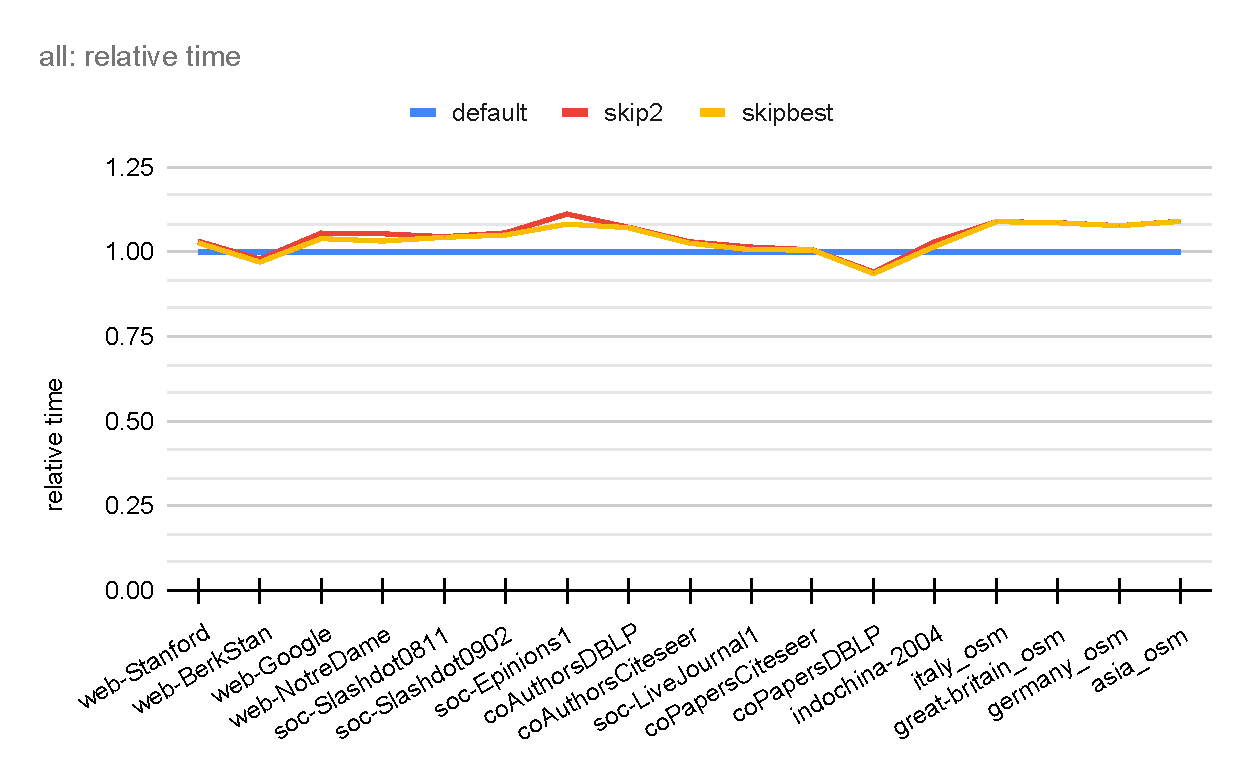
\includegraphics[width=0.48\textwidth]{out/pr-cuda-opt-c-rtime.pdf}
    \label{fig:pr-cuda-opt-c-rtime}
  }
  \subfloat{
    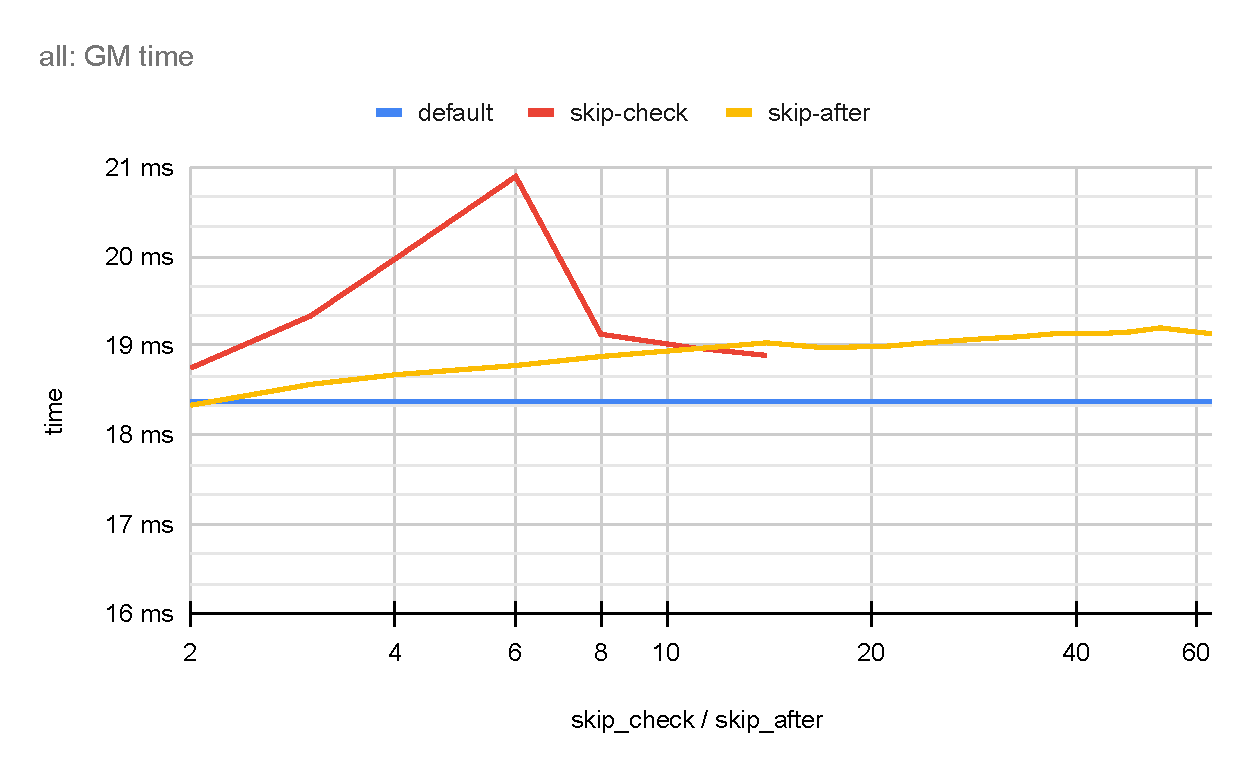
\includegraphics[width=0.48\textwidth]{out/pr-cuda-opt-d-time-gm.pdf}
    \label{fig:pr-cuda-opt-d-time-gm}
  }

  \caption{\textbf{Left:} Relative time taken for switched thread/block-per-vertex CUDA-based (GPU) static PageRank computation with the following algorithmic optimizations: no optimization (default), skip all chains (skip2), and skip chains of best min. size  (skipbest). The ratio is obtained with respect to no optimization. \textbf{Right:} GM of time taken on all graphs for switched thread/block-per-vertex CUDA-based (GPU) static PageRank computation with the following algorithmic optimizations: no optimization (none), skip converged vertices with recheck every X turns (skip-check), and skip converged vertices after X turns  (skip-after). This is relative to no optimization, with skip-check ranging from 2 to 16, and skip-check ranging from 2 to 64 (separately). Each of this is done on 5 web graphs, 4 social networks, 4 collaboration networks, and 4 road networks.}
  \label{fig:pr-cuda-opt-cd}
\end{figure*}
